\documentclass[11pt, oneside]{article} 
\usepackage{geometry}
\geometry{letterpaper} 
\usepackage{graphicx}
	
\usepackage{amssymb}
\usepackage{amsmath}
\usepackage{parskip}
\usepackage{color}
\usepackage{hyperref}

\graphicspath{{/Users/telliott_admin/Tex/png/}}
% \begin{center} 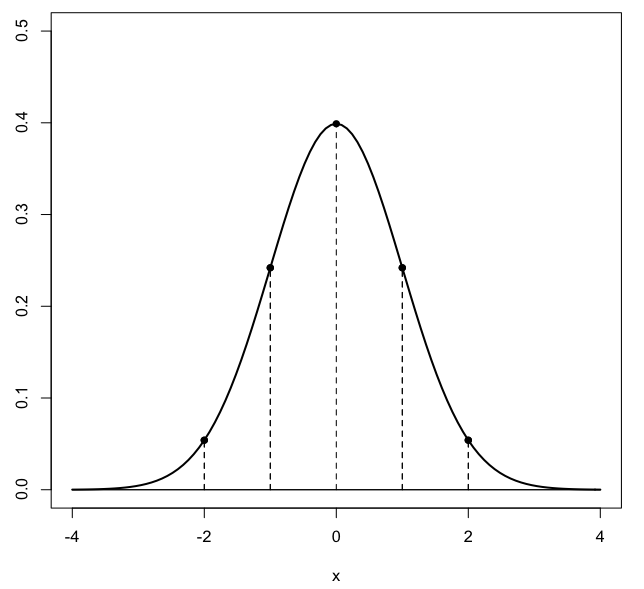
\includegraphics [scale=0.4] {gauss3.png} \end{center}

\title{History}
\date{}

\begin{document}
\maketitle
\Large

\subsection*{quadratic}

Some of the earliest examples of problems where the square root of a negative number arises involve a right triangle of a specified area and perimeter.  

Nahin says, suppose a right triangle has area $7$ and perimeter $12$.  Find the two sides.  

Label the sides as $a$ and $b$.

We can get some idea of where this problem is headed by supposing that the triangle is also isosceles with $a = b$.  Then 
\[ \frac{1}{2} ab = 7 \]
\[ ab = 14 \]
\[ a^2 = 14 \] 
so $a = \sqrt{14}$, and the perimeter is
\[ p = a + b + \sqrt{a^2 + b^2} \]
\[ = 2 \sqrt{14} + \sqrt{14 + 14} = 12.77 \]
The perimeter we are given is smaller than that

However, an isosceles right triangle has the smallest possible perimeter for a given area (the largest area for a given perimeter), hence there is no such pair $a,b$.
The problem as posed has no solution.

Proof:
Let $k$ be a constant and $x$ and $k - x$ be the given sides.  The area is
\[ A = \frac{1}{2} x (k - x) \]
\[ = -\frac{1}{2} x^2 + \frac{k}{2} x \]
The extreme point is
\[ \frac{dA}{dx} = 0 = - x + \frac{k}{2} \]
\[ x = \frac{k}{2} \]
The second derivative is $-1 < 0$, which shows that this is a minimum.  We can also see the same thing from the negative cofactor of $x^2$ in the equation.
\[ A = -\frac{1}{2} x^2 + \frac{k}{2} x \]

Doing the algebra of the original problem anyway, we solve two simultaneous equations
\[ a \cdot b = 14 \]
\[ p = a + b + \sqrt{a^2 + b^2} = 12 \]
Isolate and then remove the square root in the second one
\[ a^2 + b^2 = (12 - a - b)^2 \]
\[ = 12^2 - 12a - 12b - 12a + a^2 + ab - 12b + ab + b^2 \]
Collect terms and cancel $a^2$ and $b^2$
\[ 0 = 12^2 - 24a - 24b + 2ab \]
\[ 0 = 72 - 12a - 12b + ab \]
Substituting from the first equation given above
\[ 0 = 72 - 12a - 12 \cdot \frac{14}{a} + 14 \]
\[ 0 = 36 - 6a - 6 \cdot \frac{14}{a} + 7 \]
\[ -6 a^2 + 43a - 84 = 0 \]
\[ 6 a^2 - 43a + 84 = 0 \]

To solve this, use the quadratic formula
\[ x = \frac{-b \pm \sqrt{b^2 - 4ac}}{2a} \]
However, $b^2 = 43^2 = 1849$ is less than $4ac = 4 \cdot 6 \cdot 84 = 2016$.  We end up with
\[ x = \frac{43 \pm \sqrt{-167}}{12} \]
The classic answer at this point is just to say, these values do not exist.  The graph would be a parabola opening up ($a > 0$) whose vertex lies above the $x$-axis.

If we suppose these two \emph{complex} roots do have meaning, notice that they are what are called complex conjugates:  $p + iq$ and $p - iq$.  If they are substituted into the factored form of the quadratic:
\[ y = \ [ \ x - (p + iq) \ ] \ [ \ x - (p - iq) \ ] \]
\[ y = \ [ \ x - p - iq) \ ] \ [ \ x - p + iq) \ ] \]
\[ = x^2 - px + iqx - px + p^2 - ipq - iqx + ipq + q^2 \] 
\[ = x^2 - 2px + p^2 + q^2 \]
\[ y = (x-p)^2 + q^2 \]
$p$ is the value of $x$ at the vertex, corresponding to the minimum value of $y$, which is equal at that point to $q^2$.

Recall that the slope is
\[ y' = 2ax + b \]
at the minimum, it equals zero so
\[ 0 = 2ax + b \]
\[ x = -\frac{b}{2a} \]
This value of $x$ makes the factored form equal to zero.  It is also the first term in
\[ -\frac{b}{2a} \pm \frac{\sqrt{b^2 - 4ac}}{2a} \]

\subsection*{cubics}

In general, people just ignored problems with negative square roots  --- sometimes explicitly ---  until Cardano came to cubic polynomials.  Briefly, he discovered that any cubic like
\[ x^3 + ax^2 + bx + c = 0 \]
can be converted to a \emph{depressed} cubic of the form
\[ x^3 + px + q = 0 \]
Any cubic has either one real root and two complex ones, or else three real roots.  

We need to look at Cardano's formula to solve the depressed cubic.  He was actually solving a problem like
\[ x^3 + mx = n \]
(with $m$ and $n$ both positive), we re-write this as
\[ x^3 + mx - n = 0 \]

Define
\[ r = \frac{n}{2}, \ \ \ \  s = \frac{m^3}{27} \]

Then Cardano showed that a real root (the only one or one of the three) is
\[ x = \ [ \ r + \sqrt{r^2 + s} \ ]^{1/3} + \ [ \ r - \sqrt{r^2 + s} \ ]^{1/3} \]

Clearly, depending on the values of $m$ and $n$, and thus $r$ and $s$, $r^2 + s$ may be a negative number. 

Cardano could not just ignore this issue, because the formula works to give a real result.  He struggled with this.  

Even today, it is hard to see the resolution because of the cube root.

Write what is in the brackets as a generalized complex number, in polar format
\[ x = \ [ \ re^{i\theta} \ ]^{1/3} + \ [ \ re^{-i\theta} \ ]^{1/3} \]

Recall that complex multiplication goes like so:
\[ r_1 e^{i\theta} \ r_2 e^{i\phi} = r_1 r_2 e^{i (\theta + \phi)} \]
So a cubic is
\[ r e^{i\theta} \cdot r e^{i\theta} \cdot r e^{i\theta} = r^3 e^{i3\theta}  \]
With a change of variable, complex eponentiation is as follows:
\[ [ \ re^{i\theta} \ ]^{1/3} = r^{1/3} \ e^{i \theta/3} \]
\[ [ \ re^{-i\theta} \ ]^{1/3} = r^{1/3} \ e^{-i \theta/3} \]

The cube roots of complex conjugates are also complex conjugates!

When added together, the imaginary parts cancel, leaving an entirely real result.
\[ x = r^{1/3} \  (e^{i \theta/3} + e^{-i \theta/3}) \]

The term in brackets is clearly a sum $z + z*$, which is real, with the value twice the real component of the complex number.

\subsection*{example}
Let's figure out an example arithmetically.  The math is a little messy but we'll try to get through it.  One of the problems studied by Cardano is
\[ x^3 = 15x + 4 \]
All terms are positive, which is typical for the time.  We try the solution $x = 4$ and find it works out.  

The Tartaglia formula gives
\[ r = 4/2 = 2 \]
\[ s = (-15)^3 / 27 = -125 \]
so we have that
\[ x = \ [ \ r + \sqrt{r^2 + s} \ ]^{1/3} + \ [ \ r - \sqrt{r^2 + s} \ ]^{1/3} \]
\[ x = \ [ \ 2 + \sqrt{-121} \ ]^{1/3} + \ [ \ 2 - \sqrt{-121} \ ]^{1/3} \]

This is easy to solve if one happens to know that
\[ (2 \pm \sqrt{-1})^3 = 2 \pm \sqrt{-121} \]
Hence 
\[ x = 2 + \sqrt{-1} + 2 - \sqrt{-1} = 4 \]

Let's try to calculate this:
\[ (2 + \sqrt{-1})^3 = 2 + \sqrt{-121} \]

Usually, we would think that the polar format would make for easier calculation.  However, let's go forward using the Cartesian format
\[ (2 + i)^3 = (3 + 4i)(2 + i) \]
\[ = 6 - 4 + 11i \]
\[ = 2 + 11i \]
Pretty easy.

To use the polar format, let's compute the cube root:
\[ (2 + 11i)^{1/3} = \ ? \]
We need the polar form of $2 + 11i$.  We obtain
\[ r = \sqrt{2^2 + 11^2} = \sqrt{125} \]
\[ \theta = \tan^{-1} 11/2 =  1.391 \]
Then
\[ r' = r^{1/3} = \sqrt{5} \]
\[ \theta' = \theta/3 = 0.46346 \]

To convert back to Cartesian coordinates:
\[ x = r \cdot \cos \theta = \sqrt{5} \cdot 0.8944 = 2.0 \]
\[ y = r \cdot \sin \theta = \sqrt{5} \cdot 0.4472 = 1.0 \]
The result is $2 + i$, as expected.

\subsection*{example}

Here is another problem from Nahin showing that the real component of a complex solution may have application in the real world.

\begin{quote}Imagine that a man is running at his top speed of $v$ feet per second, to catch a bus that is stopped at a traffic light. When he is still a distance of $d$ feet from the bus, the light changes and the bus starts to move away from the running man with a constant acceleration of $a$ feet per second per second. When will the man catch the bus?
\end{quote}
 
Let the origin of coordinates be the traffic light and $x_m$ and $x_b$ be the positions of the man and the bus.  At $t = 0$, $x_b = 0$ and $x_m = - d$.  For an arbitrary time $t$
\[ x_b = \frac{1}{2} at^2 \]
\[ x_m = -d + vt \]

If the man is to catch the bus at $t = T$, the positions are the same
\[ x_m(T) = x_b(T) \]
\[ -d + vT  = \frac{1}{2} aT^2 \]

This is a quadratic
\[ \frac{1}{2} aT^2 - vT + d = 0 \]
In general, the solution for $T$ may be complex, if 
\[ v^2 - 2ad < 0 \]
Rearranging
\[ d > v^2/2a \]
For such values there is no catching the bus.  

Nahin rearranges the equation to give

\[ T^2 - 2 \frac{v}{a} T + 2\frac{d}{a} = 0 \]
The quadratic formula gives
\[ T = \frac{2v/a \pm \sqrt{4v^2/a^2 - 8d/a}}{2} \]
\[ = \frac{v}{a} \pm \sqrt{v^2/a^2 - 2d/a} \]
Even for a complex result, the real part is
\[ T = \frac{v}{a} \]

But notice:  the separation between the man and the bus is
\[ s = x_b - x_m \]
\[ = \frac{1}{2} at^2 + d - vt \]

At what time is the man closest to the bus?  That occurs when
\[ \frac{ds}{dt} = at - v = 0 \]
\[ t = \frac{v}{a} \]
This is the real part of the result above.

If the man does catch the bus ($ \sqrt{v^2/a^2 - 2d/a}$ is real), it worth thinking about the two solutions to the quadratic.  Which is the correct one and what is the meaning of the second?

\end{document}